\documentclass[11pt]{article}
\newcommand{\blind}{0}



\usepackage[nodisplayskipstretch]{setspace}
\setstretch{1}

\usepackage[utf8]{inputenc}
\usepackage{lipsum}

\usepackage{amsmath,amssymb}
\usepackage{natbib}


\usepackage{amssymb,amsbsy,amsfonts,amsmath,xspace,amsthm}
\usepackage{mathrsfs}
\usepackage{graphicx}
\allowdisplaybreaks

\usepackage{caption}
\usepackage{setspace}
\usepackage{comment}
%\doublespacing
\usepackage[margin=1in]{geometry}
\usepackage{enumitem} 
\usepackage{subcaption}
\usepackage{multirow}
\usepackage{epstopdf}
\usepackage{epsfig}
\usepackage[colorlinks,citecolor=blue]{hyperref}

\usepackage[labelfont=bf]{caption}
\usepackage{url}
\usepackage[toc,page]{appendix}
\usepackage{float}
\usepackage{natbib}
\usepackage{color}
\usepackage[dvipsnames]{xcolor}
\usepackage{verbatim}
\usepackage{authblk}
\usepackage[normalem]{ulem}


\def\ack{\section*{Acknowledgements}%
  \addtocontents{toc}{\protect\vspace{6pt}}%
  \addcontentsline{toc}{section}{Acknowledgements}%
}


\usepackage{hyperref}
\hypersetup{
    colorlinks=true,
    linkcolor=blue,
    filecolor=magenta,      
    urlcolor=cyan,
    citecolor=blue
}
 
 


\usepackage{amsmath}
\usepackage{graphicx}
\newcommand*{\KeepStyleUnderBrace}[1]{%f
\mathop{%
\mathchoice
{\underbrace{\displaystyle#1}}%
{\underbrace{\textstyle#1}}%
{\underbrace{\scriptstyle#1}}%
{\underbrace{\scriptscriptstyle#1}}%
}\limits
}
\usepackage{mathtools}
\mathtoolsset{showonlyrefs}
\usepackage{amsmath,amssymb,amsthm,bm,hyperref}
\usepackage{dsfont,listings}

 \renewcommand\footnotemark{}

\usepackage[ruled,vlined]{algorithm2e}
\SetAlFnt{\small}
\SetAlCapFnt{\small}
\SetAlCapNameFnt{\small}


\usepackage{enumitem}
\theoremstyle{plain} 
\newtheorem{thm}{Theorem}
\newtheorem{lem}{Lemma}
\newtheorem{prop}{Proposition}
\newtheorem{property}{Property}
\newtheorem{corollary}{Corollary}


\theoremstyle{definition}
\newtheorem{assumption}{Assumption}
\newtheorem{defn}{Definition}
\newtheorem{example}{Example}
\newtheorem{rmk}{Remark}
\newtheorem{clm}{Claim}

\usepackage{xcolor}
\allowdisplaybreaks
\input macros.tex

\setcounter{secnumdepth}{3}

\def\spacingset#1{\renewcommand{\baselinestretch}%
{#1}\small\normalsize} \spacingset{1}
\def\fixme#1#2{\textbf{\color{red}[FIXME (#1): #2]}}
\def\mycomment#1{\textbf{\color{blue}#1}}
\def\ccomment#1{\textbf{\color{ForestGreen}#1}}
\usepackage{hyperref}
\usepackage[parfill]{parskip}
\usepackage{bm}


\newcommand{\Hnorm}[1]{\left\lVert#1\right\rVert_{\tH_\alpha}}
\newcommand{\nullnorm}[1]{\left\lVert#1\right\rVert}
\def\trueB{\mB^{\text{true}}}
\def\newX{\mX_{\textup{new}}}
\def\newy{y_{\textup{new}}}
\def\sign{\textup{sign}}
\def\bayesf{f_{\textup{bayes}}}
\def\bayesS{S_{\textup{bayes}}}
\def\bayespif{f_{\textup{bayes},\pi}}
\def\CNN{\text{\bf \small CNN }}
\def\Lasso{\text{\bf \small Lasso }}
\def\NonparaM{\text{\bf \small NonMAR }}
\def\LogisticM{\text{\bf \small LogisticM }}
 
 

\usepackage{setspace}
\onehalfspacing
 
\begin{document}

\if1\blind
{   \date{}
  \title{\bf Nonparametric learning with matrix-valued predictors in high dimensions}
\author{ Chanwoo Lee$^{1}$, Lexin Li$^2$, Hao Helen Zhang$^3$, and Miaoyan Wang$^1$\footnote{
\hspace*{-.6cm}$^1$Department of Statistics, University of Wisconsin-Madison\\
$^2$Department of Biostatistics and Epidemiology, University of California at Berkeley\\
$^3$Department of Mathematics, University of Arizona}
}

    \maketitle
} \fi

\if0\blind
{
 \date{}
  \title{\bf Nonparametric learning with matrix-valued \\predictors in high dimensions}
\author{}
\maketitle
} \fi

\begin{abstract}
We consider the problem of learning the relationship between a binary label response and a high-dimensional matrix-valued predictor. Prediction based on matrices or networks has recently surged in brain connectivity studies, sensor network localization, and integrative genomics. Traditional regression methods take a parametric procedure by imposing a priori functional form between variables. These parametric models, however, are inadequate for structure learning and often fail in accurate prediction. Here, we develop a learning reduction framework to address a range of learning tasks from classification to regression for matrix-valued predictors. Our proposal achieves interpretable prediction via a low-rank two-way sparse representation of the target function. Unlike earlier approaches, our method automatically learns and exploits the important features in the high-dimensional matrices. Statistical accuracy, excess risk bounds, and efficient algorithms are established. We demonstrate the advantage of our method over previous approaches through simulations and applications to human brain connectome data. 

\end{abstract}
\noindent%
{\it Keywords:}  Nonparametric learning, high-dimensional matrices, sparse and low-rank models, classification, regression, feature selection

\section{Introduction }

Matrix-valued predictors ubiquitously arise in modern applications. In brain connectivity studies, for example, individuals are represented by their brain networks, and the networks quantify the connectivity patterns over a set of nodes (brain regions of interest). Human connectom project~\citep{wang2019common} has constructed brain networks for over 1,200 individuals using Desikan atlas with 68 brain nodes. Structural connectivity is measured for every pair of nodes, resulting in an adjacency matrix of size 68 $\times$ 68 for each individual. This connectivity matrix provides important information for disease prediction. Other examples include electroencephalography studies of alcoholism~\citep{zhou2014regularized}. Researchers measure the voltage values from 64 channels of electrodes on 256 subjects for 256 time points. The study yields a $256 \times 64$ matrix-valued feature, along with a binary indicator of subject being alcoholic or not. Identifying the relationship between EEG signals and alcoholism is helpful for disease diagnostics. 


We consider the statistical learning problem of modeling the relationship between a matrix-valued predictor $\mX \in \mathbb{R}^{d_1\times d_2}$ and a binary label response $y\in\{-1,1\}$.  The key challenge with matrix-valued predictors is the high-dimensional multi-way structure in the feature space. One possible approach is to transform the predictors into vectors and apply classical methods such as Lasso \citep{friedman2010regularization}. The practice of vectorization, however, destroys the structural information in the original predictors. Indeed, network data encoded as matrices represent various aspects of features, including global structure (e.g.\ clustering patterns, community hubs) and local structure (e.g.\ node degrees, edge connections). Learning and incorporating these features are important for prediction. There have been several recent attempts to allow matrix-valued predictors; for example, trace regression~\citep{fan2019generalized}, network logistic regression~\citep{relion2019network}, and matrix linear discriminant analysis~\citep{hu2020matrix}. These parametric approaches impose a priori functional form between variables and often lead to inaccurate prediction in high dimensions. For these reasons, nonparametric approaches such as $k$-nearest neighbors, decision trees, and convolutional neural network (CNN) have been popular. Current nonparametric methods aim for accurate prediction at the cost of hard interpretability. In our motivating brain network application and many other scientific studies, however, researchers are interested in {\it interpretable prediction}, where the goal is to not only make accurate prediction but also identify most informative features for descriptive simplicity. Efficient methods that achieve both have yet to be developed. 
 


{\bf Our contributions.} We develop a nonparametric method that automatically exploits the matrix-valued feature space for accurate prediction. We address three matrix problems -- classification, level set estimation, and regression -- via a learning reduction approach. The proposal achieves interpretable prediction using a low-rank two-way sparse representation of the target functions. We establish convergence guarantees in high dimensions that permit the matrix dimension to grow with sample size. Unlike earlier approaches, our method performs efficient variable selection and adapts to the possibly non-smooth, non-linear functions of interest. Our numerical analyses and application demonstrate the outperformance of the proposed approach over previous methods. 


 
{\bf Notation.} Let $\tX=\mathbb{R}^{d_1\times d_2}$ be the feature space. Given a function $f\colon \tX \to \mathbb{R}$, we use $\sign f$ to denote its sign function, such that $\sign f(\mX)=1$ if $f(\mX)>0$ and $\sign f(\mX)=-1$ otherwise. The notion of sign function also extends to sets in $\tX$. We use $\sign (\mX\in A)$ to denote the sign function induced by the set $A\subset\tX$, i.e.,\ a function taking value $1$ on the event $\{\mX\in A\}$ and -1 otherwise. We use shorthand $[n]:=\{1,\ldots,n\}$ to denote the $n$-set for $n\in\mathbb{N}_{+}$ and use $|\cdot|$ to denote the cardinality of sets. Let $\newnormSize{}{\cdot}_p$ denote the vector $p$-norm for $p\geq 0$, and $\FnormSize{}{\cdot}$ be the matrix Frobenious norm. Given a $d_1$-by-$d_2$ matrix $\mB$, we use $\mB_i$ to denote the $i$-th row of $\mB$. The $(p,q)$-norm of a matrix $\mB$ is defined as $\newnormSize{}{\mB}_{p,q}=\newnormSize{}{\mb}_q$, where $\mb=(\newnormSize{}{\mB_1}_p,\ldots,\newnormSize{}{\mB_{d_1}}_p)^T\in\mathbb{R}^{d_1}$ consists of the $p$-norms for each of the rows in $\mB$. In particular, $\newnormSize{}{\mB}_{1,0}=|\{i\in [d_1]\colon \mB_i\neq 0\}|$ denotes the number of non-zero rows in $\mB$. An event $E$ is said to occur ``with high probability'' if $\mathbb{P}(E)$ tends to 1 as the matrix dimension $d_{\min}=\min(d_1,d_2)\to\infty$. We denote $a_n\asymp b_n$ if $\lim_n b_n/a_n\rightarrow c$ for some constant $c>$ and denote $a_n\lesssim b_n$ if $\lim_n b_n/a_n\rightarrow 0.$ We use $\mathds{1}(\cdot)$ to denote the indicator function. 

\section{Three learning problems}

We present the main learning goals of our interest. Let $\mX\in\mathbb{R}^{d_1\times d_2}$ denote the matrix-valued predictor, $y\in\{-1,1\}$ denote the binary label response, and $\mathbb{P}_{\mX,y}$ denote the unknown joint probability distribution over the pair $(\mX,y)$. In the context of binary response, $y$ is a Bernoulli random variable with conditional probability $p(\mX)\stackrel{\text{def}}{=}\mathbb{P}(y=1|\mX)$; we generally make no parametric assumptions on the marginal distribution $\mathbb{P}_{\mX}$ or form of $p(\mX)$. 


Suppose that we observe a sample of $n$ training data points, $(\mX_1,y_1),\ldots,(\mX_n,y_n)$, identically and independently distributed (i.i.d.) according to $\mathbb{P}_{\mX,y}$. Let $(\mX_{\text{new}},y_{\text{new}})$ be a future unseen test point drawn independently from the same distribution. Our goal is to predict $y_{\text{new}}$ based on $\mX_{\text{new}}$. We often omit the subscript ``new'' and simply write $(\mX,y)$ for the prototypical test point. The relevant probabilistic statements should be interpreted as taken jointly with respect to $(\mX,y)$.

We consider three learning problems: classification, level set estimation, and regression. 

\begin{enumerate}[label={2.\arabic*},wide, labelwidth=!, labelindent=0pt]
\item {\it Matrix classification}: Classification is the problem of predicting the label $y\in \{-1,1\}$ to which the new matrix $\mX$ belongs. A prediction rule (also called a classifier) decides that $y=1$ if $\mX\in S$ and $y=0$ if $\mX \not\in S$, where $S$ is a Borel subset of $\mathbb{R}^{d_1\times d_2}$. We formulate the classification problem as choosing a classifier $S\in \tS$, from a given set of candidate classifiers $\tS$, that minimizes the expected classification error 
\begin{equation}\label{eq:classloss}
R(S)=\mathbb{P}_{\mX,y}\left[y\neq \sign(\mX\in S)\right].
\end{equation}
The $R(S)$ is also called the classification risk. When the candidate set $\tS$ consists of all Borel subsets of $\mathbb{R}^{d_1\times d_2}$, the minimizer of~\eqref{eq:classloss} is called the Bayes classifier. It is known that the Bayes classifier can be written as 
\begin{equation}\label{eq:bayes}
\bayesS=\{\mX\in\mathbb{R}^{d_1\times d_2}\colon p(\mX)\geq 1/2\}.
\end{equation}
The expression~\eqref{eq:bayes} is one of many equally good Bayes classifiers, because arbitrary prediction rules are allowed on the boundaries $\partial S_{\text{bayes}} = \{\mX\colon p(\mX)=1/2\}$. Without loss of generality, we will use~\eqref{eq:bayes} as the canonical form of the Bayes classifier. 


In practice the population distribution is unknown, so the objective function~\eqref{eq:classloss} and the minimizer needs to be estimated through the data $\{\mX_i,y_i\}_{i\in[n]}$. Our first goal is to estimate the Bayes classifier for matrix classification. 

{\bf Question 1.} How to perform classification when matrix dimension far exceeds the sample size $n$?

\item {\it Level set estimation}: The problem of level set estimation generalizes the classification task. For a given $\pi\in(0, 1)$, the target $\pi$-level set of the conditional probability function $p(\mX)$ is defined as
\begin{equation}\label{eq:level}
\bayesS(\pi) = \{\mX\in\mathbb{R}^{d_1\times d_2}\colon p(\mX)\geq \pi\}.
\end{equation}
An important fact is that the set $\bayesS(\pi)$ optimizes the weighted classification risk~\citep{willett2007minimax,scott2007regression,wang2008probability}. Specifically, among all Borel subsets of $\mathbb{R}^{d_1\times d_2}$, the set $S_{\text{bayes}}(\pi)$ is the global minimizer of the expected $\pi$-weighted classification error,
\begin{equation}\label{eq:risklevel}
R_\pi(S)=\mathbb{E}\left[ w_{\pi}(y)\mathds{1}(y\neq \sign(\mX\in S))\right],
\end{equation}
where we define $w_{\pi}(y)=1-\pi$ or $\pi$ depending on $y=1$ or $-1$. In light of~\eqref{eq:classloss} and~\eqref{eq:risklevel}, the level set estimation is an extension of the usual classification from equal weight $\pi=1/2$ to general weight $\pi \in(0,1)$. Accurate level set estimation plays an important role in applications of geographical elevation maps, imaging contour detection, and motion tracking. We consider the following question:

{\bf Question 2.} How to simultaneously estimate the level set and identify important variables in the matrix-valued predictor space, for the goal of interpretable prediction?


\item {\it Nonparametric regression}: The problem of nonparametric regression is to estimate the conditional mean $\mathbb{E}(y|\mX)$ as a multivariable function in the predictor space. In the our contexts, the nonparametric regression is equivalent to estimating the conditional probability $p(\mX)=\mathbb{P}(y=1|\mX)=\frac{1}{2}(\mathbb{E}(y|\mX)+1)$. Throughout the paper we will focus on $p(\mX)$ and refer to it as the regression function. 
The function $p(\mX)$, is the global minimizer, among all measurable functions $f\colon \mathbb{R}^{d_1\times d_2}\to[0,1]$, to the expected squared error,
\begin{equation}\label{eq:regression}
R_{\text{reg}}(f)=\mathbb{E}\left[y+1-2f(\mX)\right]^2,
\end{equation}
where $R_{\text{reg}}(f)$ is also known as regression risk. Our final goal is the function estimation:

{\bf Question 3.} How to learn the regression function $p(\mX)$ in the high-dimensional matrix space?
\end{enumerate}


\begin{figure}\centering
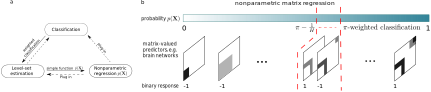
\includegraphics[width=1\textwidth]{new_demo.pdf}
\caption{(a) Our learning reduction approach (solid line) to the three problems of interest. The classical plug-in approaches are depicted in dashed line. (b) Matrix nonparametric regression via $\pi$-weighted classification.}\label{fig:diagram}
\end{figure}

The three problems of our interest represent a range of learning tasks with increasing difficulties. Classification is a special case of level set estimation with $\pi=1/2$, whereas the level set is a discrete approximation of the regression function. A common approach is to address regression first, and then solve the earlier two using plug-in estimates (Figure~\ref{fig:diagram}a). This procedure, however, undermines the fact that regression is generally harder than the other two. Indeed, as we show in Section~\ref{sec:theory}, regression has a slower convergence rate $\tO(n^{-1/2})$ compared to the rate $\tO(n^{-1})$ of classification. Ignorance of the increased complexity violates Vapnik’s maxim: \emph{When solving a given problem, one should try to avoid solving a more general problem as an intermediate step.} 

\section{From classification to regression: a new deal}\label{sec:idea}
We develop a ``learning reduction'' approach (Figure~\ref{fig:diagram}a) by relating the regression to classification, the latter of which is more fundamental and easier. We addresses classification first and use the results to solve the regression. In general, regression requires more assumptions than classification. Our learning reduction approach bridges these two tasks using level set estimation, a problem lies somewhere in between. The connection allows us to disentangle complexity and leverage existing algorithms. 

In this section we restrict our attention to the population properties of regression function $p(\mX)$ when the true distribution $\mathbb{P}_{\mX,y}$ is known. This simplified situation leads to a cleaner characterization with deterministic risk functions in~\eqref{eq:classloss}, \eqref{eq:risklevel}, and \eqref{eq:regression}. The finite sample estimation will be presented in Section~\ref{sec:theory}, in which we address the general case with unknown distribution $\mathbb{P}_{\mX,y}$, and the only information is through empirical (stochastic) risk estimated from the training set $(\mX_i,y_i)_{i=1}^n$. 


\subsection{Level set approaches to nonparametric matrix regression}\label{sec:bridge}
Figure~\ref{fig:diagram}b illustrates the main idea of our approaches. We use a sequence of weighted classifications to find the level sets in the matrix space, and then estimate the regression function $p(\mX)=\mathbb{E}(y=1|\mX)$ via level set aggregation. Our building block is to use level sets to estimate regression function $p$ through classifications. The level set approach bridges the two sides of a same coin -- characteristic (set indicator) functions in functional analysis and weighted classifications in statistical learning. 

Specifically, let $p(\cdot)\colon \mathbb{R}^{d_1\times d_2}\to [0,1]$ be the target regression function of interest, and $\bayesS(\pi)=\{\mX\colon p(\mX)\geq \pi\}$ be the associated $\pi$-level set. Let $\Pi=\{{1\over H}, {2\over H}, \ldots, {H-1\over H} \}$ be a sequence of evenly spaced points in $[0,1]$, where $H\in\mathbb{N}_{+}$ is the resolution parameter. We introduce an $H$-step function $\bar p(\cdot)\colon \mathbb{R}^{d_1\times d_2} \to [0,1]$ by
\begin{equation}\label{eq:stepfunction}
\bar p(\mX)= {1\over 2H}  \sum_{\pi \in \Pi} \sign (\mX\in \bar S(\pi))+{1\over 2}, \quad \text{for all }\mX\in\mathbb{R}^{d_1\times d_2},
\end{equation}
where, for every $\pi\in\Pi$, the set $\bar S(\pi)\subset \mathbb{R}^{d_1\times d_2}$ is the classifier that minimizes the $\pi$-weighted classification risk,
\begin{equation}\label{eq:constrained}
\bar S(\pi) \stackrel{\text{def}}{=} \argmin_{S\in \tS}R_\pi(S), \quad \text{where}\quad R_\pi(S)=\mathbb{E}\left[ w_{\pi}(y)\mathds{1}(y\neq \sign (\mX\in S))\right],
\end{equation}
subject to the constraint $S\in\tS$, with $\tS$ being a given candidate set of classifiers. When the set $\tS$ is rich enough, e.g., $\tS$ consists of all Borel sets, then $\bar S(\pi)$ has the same risk as $\bayesS(\pi)$. We leave the $\tS$ in general here; the specific choice of $\tS$ will be described in Section~\ref{subsec:linear class}. 

In order to address the accuracy between $\bar p(\mX)$ and $p(\mX)$, we need to establish the identification of level sets $S(\pi)$ from optimization~\eqref{eq:constrained}. The Bayes classifier $\bayesS(\pi)$ minimizes the weighted classification risk $R_\pi(S)$; the inverse may not be true because of possible multiple global minimizers of $R_\pi(S)$ even in the ideal scenario with no constraints on $\tS$. The uniqueness and stability around $\bayesS(\pi)$ turns out to play a key role for the accurate estimation of $p(\mX)$. 

We introduce the following notion to characterize the behavior of the regression function near the level set boundaries $\partial S_{\text{bayes}}(\pi) = \{ p(\mX)= \pi\}$. The condition essentially quantifies the uniqueness of level sets recovery from weighted classification.

\begin{defn} [Global regularity]\label{ass:decboundary}We call a level $\pi\in[0,1]$ a mass point if the level set boundary $\partial \bayesS(\pi)$ has non-zero measures under $\mathbb{P}_{\mX}$. Let $\tN=\{\pi\in[0,1] \colon \mathbb{P}\left[p(\mX)=\pi\right]\neq 0\}$ denote the collection of mass points in $p(\mX)$. A function $p(\mX)$ is called $\alpha$-globally regular with $\alpha\in[0,1]$, if 
\begin{enumerate}[label=(\roman*),wide, labelwidth=!, labelindent=0pt,topsep=-5pt,itemsep=-1ex,partopsep=0ex,parsep=1ex]
\item $p(\mX)$ has finitely many mass points, i.e., $|\tN|\leq C'$ for some constant $C'<\infty$; and 
\item 
there exists a global constant $C>0$ such that, for all $\pi \notin \tN $,
\begin{equation}\label{eq:mass}
\mathbb{P}_{\mX}(|p(\mX)-\pi|\leq t)\leq Ct^{\alpha/(1-\alpha)}, \quad \text{for }t\in \left(0,\rho(\pi,\tN)\right),
\end{equation}
where $\rho(\pi,\tN)\stackrel{\text{def}}{=}\min_{\pi'\in \tN} |\pi-\pi'|$  denotes the distance from $\pi$ to the nearest mass point in $\tN$. When $\tN = \phi$, we define $\rho(\pi,\tN)=1$. When $\alpha=1$, the right-hand-side of~\eqref{eq:mass} is interpreted as zero.
\end{enumerate}
\end{defn}

Definition~\ref{ass:decboundary} controls the uniform behavior of $p(\mX)$ across possible $\pi$. If the condition~\eqref{eq:mass} holds for a fixed $\pi$, we call the function $p(\mX)$ is $(\pi,\alpha)$-locally regular. The exponent $\alpha$ quantifies the concentration of probability mass $p(\mX)$ around level set boundaries.

We show that Definition~\ref{ass:decboundary} implies the global identifiability of $\bayesS(\pi)$ from optimization \eqref{eq:constrained} across all $\pi\notin \tN$.
For two sets $S_1, S_2 \in \mathbb{R}^{d_1\times d_2}$, we define the probabilistic set difference 
\begin{align}\label{eq:riskdiff}
d_{\Delta}(S_1,S_2)\stackrel{\text{def}}{=}\mathbb{P}_{\mX}(S_1\Delta S_2)=\mathbb{P}_{\mX}\{\mX\colon \mX\in S_1\setminus S_2 \text{ or }S_2\setminus S_1\},
\end{align}
and the risk difference
\begin{align}\label{eq:setdiff}
d_\pi(S_1,S_2)\stackrel{\text{def}}{=} R_{\pi}(S_1)-R_{\pi}(S_2).
\end{align}

\begin{thm}[Identifiability]~\label{thm:identifiability} Suppose the regression function $p(\mX)$ is $\alpha$-globally regular with $\alpha\in[0,1]$. Then, there exists a constant $c>0$ such that
\begin{align}\label{eq:identity}
d_{\Delta}(S,\bayesS(\pi)) \leq c\left[d_\pi^\alpha(S,\bayesS(\pi))+{1\over\rho(\pi, \tN)} d_\pi(S,\bayesS(\pi))\right],
\end{align}
for all sets $S\in\mathbb{R}^{d_1\times d_2}$ and levels $\pi\notin \tN$.
\end{thm}

The bound~\eqref{eq:identity} controls the worst-case perturbation of classifiers in the probability space $\mathbb{P}_{\mX}$ with respect to weighted classification risks. When $\alpha\neq 0$, the inequality~\eqref{eq:identity} immediately implies the uniqueness of $\bayesS(\pi)$ up to a measure-zero set in $\mathbb{P}_{\mX}$ whereas $\alpha=0$ corresponds to no identifiability.  Notice that $\rho(\pi,\tN)$ becomes a constant for fixed $\pi$, implying that local regularity ensures the identifiability of Bayes set $\bayesS(\pi)$.


Our identifiability conclusion generalizes the earlier result for single level set estimation~\citep{singh2009adaptive,tsybakov2004optimal}. Inspection of the proof shows that the set estimation is more difficult at levels where the point mass concentrates (small $\alpha$), as intuition would suggest. Consider a simple case when the entries of matrix $\mX$ are i.i.d.\ drawn from $\text{Uniform}[-1,1]$; that is, $\mathbb{P}_{\mX}$ is the Lebesque measure on $[0,1]^{d_1d_2}$. Then, the best rate $\alpha\to 1$ corresponds to a clear separation with no point mass at the boundary, whereas the worst rate $\alpha\to 0$ corresponds to a heavy mass of $p(\mX)$ near the boundary. A typical intermediate case is $\alpha=1/2$ when $p(\mX)$ has non-degenerate first-order Taylor expansion around $\pi$. We omit the proof for space considerations.

Now we reach the main result of this section by putting together the proposal~\eqref{eq:stepfunction},~\eqref{eq:constrained} and Theorem~\ref{thm:identifiability}. Define the regression excess risk by $R_{\textup{reg}}(\bar p) - R_{\textup{reg}}(p)$.
The following result bounds the regression excess risk using classification excess risk.

\begin{thm}[Nonparametric regression via weighted classifications]\label{thm:twobounds} Suppose that the regression function $p(\mX)$ is $\alpha$-globally regular with $\alpha\in[0,1]$. Let $\bar p(\mX)$ the step function constructed from weighted classifiers as in~\eqref{eq:stepfunction}. Then, there exists a constant $c_1,c_2>0$ such that
\begin{align}\label{eq:approximation}
R_{\textup{reg}}(\bar p) - R_{\textup{reg}}(p)&\leq 4\mathbb{E}_{\mX}\left| \bar p(\mX)- p(\mX)\right|\notag\\
&\leq {2\over H}+ \frac{4}{H}\sum_{\pi\in\Pi}\left\{d_\pi^{\alpha}(\bayesS(\pi),\bar S(\pi))+ H d_\pi(\bayesS(\pi),\bar S(\pi))\right\}.
\end{align}
for all resolution parameter $H=|\Pi|\in \mathbb{N}_{+}$. 

\end{thm}

Theorem~\ref{thm:twobounds} shows the key role of $\bar p(\mX)$ in bridging regression and classification. The results suggest that the estimation of $p(\mX)$ can be reduced to estimation of $\bar p(\mX)$, or equivalently, to a sequence of weighted classifications $\{\bar S(\pi)\}_{\pi\in\Pi}$. The regression excess risk bound~\eqref{eq:approximation} has two terms. The first term is the bias due to the step function approximation to the regression function. The second term is the excess risk for classification optimized over $\tS$ compared to that over all Borel sets, representing the capability of the candidate classifiers $\tS$. In the case of unknown population risk $R_\pi(\cdot)$, the second term should be plugged in using the empirical risk, which results in an additional variance term due to finite sample size. The resolution parameter $H$ shall be chosen to balances the bias-variance tradeoff. 

Estimating $\bar p(\mX)$ as a surrogate of $p(\mX)$ provides several benefits. From a computational perspective, $\bar p(\mX)$ is a finite combination of weighted classifiers, which are easier to solve than a direct regression. From the statistical perspective, the function $\bar p(\mX)$ provides a valid approximation to $p(\mX)$ even when $p(\mX)$ is non-smooth and irregular. In particular, the estimation accuracy relies little on the local neighborhood of $\mX$ but rather on the local neighborhood of $p(\mX)$. Note that the former is a $d_1d_2$-dimensional random variable whereas the later is a $[0,1]$-valued univariate random variable. The shifted focus of local structure to the range space is especially appealing for matrix-valued predictors, since the predictor space is high dimensional and often barely explored by small sample size data.  

\subsection{Sparse and low-rank function boundaries}\label{subsec:linear class}
We describe the choice of candidate classifiers $\tS$ in~\eqref{eq:constrained}. We rewrite the optimization~\eqref{eq:constrained} as the minimization over continuous-valued functions,
\begin{equation}\label{eq:optimization}
\bar S(\pi) = \{\mX\colon\bar f(\mX)\geq 0\},\quad  \text{with}\quad  \bar f(\mX)= \argmin_{f\in\tF}\mathbb{E}\left[w_\pi(y)\mathds{1}(y\neq \sign f(\mX))\right],
\end{equation}
where $\bar f\in\tF$ is a continuous-valued function from $\mathbb{R}^{d_1\times d_2}$, and its sign induces the classifier $\bar S(\pi)\in\tS$. The choice of $\tS$ thus reduces to the choice of function family $\tF$. A desirable $\tF$ should balance the prediction and interpretability; i.e., $\tF$ should be flexible enough for accurate prediction while being simple enough for high interpretability. 

We propose the linear function family $\tF$ with low-rank two-way sparse matrix coefficients,
\begin{align}\label{eq:class}
\tF(r,s_1,s_2)=\{f\colon \mX\mapsto \langle \mX, \mB \rangle +b \ \big|\ \text{rank}(\mB)\leq r, \ \text{supp}(\mB)\leq (s_1,s_2), \ \mB\in\mathbb{R}^{d_1\times d_2},\ b\in\mathbb{R}\},
\end{align}
where $\text{rank}(\mB)$ denotes the rank of the coefficient matrix, and $\text{supp}(\mB)$ denotes the two-way sparsity parameter with $s_1=\newnormSize{}{\mB}_{1,0}$ and $s_2=\newnormSize{}{\mB^T}_{1,0}$ being the numbers of non-zero rows and columns of $\mB$, respectively. For the theory, we assume that $(r,s_1,s_2)$ are known; the adaptation to unknown $(r, s_1, s_2)$ in practice is described in Section~\ref{sec:data}.  
Combining formulations~\eqref{eq:stepfunction},~\eqref{eq:optimization} and~\eqref{eq:class} yields our (population version) ``learning deduction'' approach to nonparametric matrix regression.


The low-rank two-way sparse classifier~\eqref{eq:class} enables efficient variable selection in high-dimensional matrices, thereby achieving high interpretability in prediction. In the brain network analysis, scientists are interested in identifying important nodes attached to at least one active edges with non-zero effects. Classical entrywise sparsity essentially treats $\mX$ as ``a bag of non-ordered edges'', and loses the two-way paring information among entries. In contrast, our two-way sparsity efficiently identifies the underlying active nodes by making use of matrix structure in the predictors. 

It is worthy noting that the linearity in the classifiers $\tF$ does not preclude the global nonlinearity in the regression function $p(\mX)$ or its variant $\bar p(\mX)$. As shown in the following examples, many nonlinear regression functions in existing literature are special cases of our representation~\eqref{eq:optimization} with~\eqref{eq:class}, in the sense that the second term in the approximation~\eqref{eq:approximation} becomes precisely zero. 

\begin{example}[Single index models~\citep{alquier2013sparse,ganti2017learning}]\label{example:1}
Suppose the true regression function can be expressed as $p(\mX)= g(\langle \mX,\mB\rangle)$, where $g(\cdot)\colon \mathbb{R}\to [0,1]$ is an arbitrary monotonic function, and $\mB$ is a low-rank two-way sparse matrix. Then, for every $\pi\in(0,1)$, there exists $f\in \tF(r,s_1,s_2)$, such that $\sign(p(\mX)-\pi)= \sign f(\mX)$. Our method generalizes single index model to high dimensional matrices by joint learning matrix coefficient $\mB$ and nonlinear function $g$. 
\end{example}

Common link functions, such as logistic function $g(t)=(1+\exp(-t))^{-1}$, arctangent function $g(t)={1\over \pi}\arctan(t)+{1\over 2}$, truncated rectified linear unit (ReLU) function $g(t)=t\mathds{1}(t\in[0,1])+\mathds{1}(t>1)$, and any arbitrary inverse cumulative distribution functions are included in our functional class. In particular, our model generalizes the matrix regressions~\citep{zhou2014regularized,guha2020bayesian,relion2019network} to the case with unknown link functions. 

Our function class also incorporates models from matrix linear discriminant analysis (LDA)~\citep{hu2020matrix}. 

\begin{example}[Multivariate normal mixtures~\citep{hu2020matrix}] Suppose the matrix-valued predictor $\mX$ follows a Gaussian mixture distribution, $\mX|\{y=-1\}=\mB_1+\mE_1$ and $ \mX|\{y=1\}=\mB_2+\mE_2$, where $(\mB_1-\mB_2)$ is a low-rank two-way sparse matrix, and $\mE_1, \mE_2$ are two mutually independent noise matrices with i.i.d.\ $N(0,1)$ entries. Then, for every $\pi\in(0,1)$, $\sign(p(\mX)-\pi)= \sign f(\mX)$ for some $f\in \tF(r,s_1,s_2)$. More generally, we have established the characterization by extending two classes of $\mX$ to a series of $\mX=\mX(\pi)$ over a continuous spectrum of $\pi \in (0,1)$ (results not shown). 
\end{example}

In principle, more complicated classifiers, such as neural network, decision trees, and boosting, can also be brought to bear on the level set construction~\eqref{eq:optimization}. The ability to import and adapt existing classification methods is one advantage of the proposed learning reduction framework. We find that, in our motivating brain network analysis, the low-rank two-way sparse classifiers~\eqref{eq:class} provide the benefit of interpretable predictions (see Section~\ref{sec:real}). 

\section{Estimation}\label{sec:theory}
In previous sections we have established the population properties from classification to regression (Figure~\ref{fig:diagram}b). In this section we address the empirical learning problems when the true distribution $\mathbb{P}_{\mX,y}$ is unknown. The objective function in the earlier optimization now becomes empirical (stochastic) risks calculated from high dimensional low sample size training data $(X_i,y_i)_{i=1}^n$. 

\subsection{Large-margin learning with high dimensional matrices}
When the distribution $\mathbb{P}_{\mX,y}$ is unknown, we propose the regression function estimate $\hat p(\cdot)\colon \mathbb{R}^{d_1\times d_2} \to [0,1]$ by
\begin{equation}\label{eq:stepfunctionsample}
\hat p(\mX)= {1\over 2H}  \sum_{\pi \in \Pi} \sign (\mX\in \hat S(\pi))+{1\over 2},\quad \text{for all }\mX\in\mathbb{R}^{d_1\times d_2}.
\end{equation}
Here, for every $\pi\in\Pi$, the set $\hat S(\pi)\subset \mathbb{R}^{d_1\times d_2}$ is the estimated classifier from empirical surrogate risk minimization,

\begin{align}\label{eq:large-margin}
\hat S(\pi) = \{\mX \colon \hat f_\pi(\mX) \geq 0\}, \quad \text{with}\quad \hat f_\pi=\min_{f\in\tF(r,s_1,s_2)}\left\{ {1\over n}\sum_{i=1}^n w_{\pi}(y_i)\ell\left(y_if(\mX_i)\right)+ \lambda \FnormSize{}{f}^2\right\},
\end{align}
where $w_\pi(y) = 1-\pi $ if $y = 1$ and $w_\pi(y)=\pi$ if $y = -1$ is the label-dependent weight; $\ell(z)\colon \mathbb{R}\mapsto \mathbb{R}_{\geq 0}$ is the surrogate classification loss defined as a function of margin $z=yf(\mX)$; $\lambda>0$ is the penalty parameter; and we define the penalization term $\FnormSize{}{f}=\FnormSize{}{\mB}$, with $\mB$ being the coefficient matrix associated with $f\in\tF(r,s_1,s_2)$. Examples of large-margin loss functions are hinge loss $\ell(z) = (1-z)_+$ for support vector machines, logistic loss $\ell(z) =\log(1+e^{-z})$ for important vector machines, and $\psi$-loss $\ell(z)=2\min(1,(1-z)_+)$ with $z_{+}=\max(z,0)$. We choose hinge loss for parsimony; our framework applies equally to other common large-margin losses~\citep{bartlett2006convexity}. 

The estimation~\eqref{eq:large-margin} generalizes the population formulation~\eqref{eq:optimization} from three aspects. First, the population expectation in~\eqref{eq:optimization} is replaced by the empirical sample average, which is common in statistical learning problems with i.i.d.\ assumption. Second, we add the ridge penalization $\lambda\FnormSize{}{f}^2$ to control the magnitude of the classifiers. The oracle tuning parameter $\lambda$ depends on the sample size and the problem dimension as we will describe in the next paragraph. The resulting sieve estimate enjoys numerical stability and statistical accuracy. In practice, we choose $\lambda$ in a data-adaptive fashion via cross validation. Third, we replace the binary loss in~\eqref{eq:optimization} by a more manageable large-margin loss. This relaxation allows us to leverage efficient large-margin algorithms while maintaining desirable statistical performance under mild assumptions. 


\subsection{Alternating optimization for structural risk minimization}
We describe the optimization algorithm for solving matrix classification and regression. We focus on the general $\pi$-weighted classification~\eqref{eq:large-margin} because both classification and regression naturally follow by setting $\pi={1\over 2}$, and $\pi\in\{{1\over H},\ldots,{1-H\over H}\}$, respectively. For brevity, we assume the intercept in the function class~\eqref{eq:class} is zero, and use $\tF(r,s_1,s_2)$ to denote the set of matrices satisfying $\text{rank}(\mB)\leq r$ and $\text{supp}(\mB)\leq (s_1,s_2)$. The estimation problem~\eqref{eq:large-margin} is formulated as an optimization over matrix space,
\begin{equation}\label{eq:sampleoptim}
\min_{\mB \in \tF(r,s_1,s_2)}L(\mB),\quad \text{where }L(\mB)={1\over n}\sum_{i=1}^nw_\pi(y_i)\ell(y_i\langle \mX_i,\mB \rangle) + \lambda\FnormSize{}{\mB}^2,
\end{equation}
where the objective function can be either convex (such as hinge loss, logistic loss) or non-convex ($\psi$-loss). The optimization~\eqref{eq:sampleoptim} has a non-convex feasible region because of the low-rank and sparse constraint. 

We propose an alternating direction method of multipliers (ADMM) approach to solve problem of this type. ADMM introduces a dual variable and an additional feasibility constraint to perform coordinate descent in the corresponding augmented Lagrangian function. The augmented ADMM objective in our context is given by
\begin{equation}\label{eq:ADMM}
L(\mB,\mS,\mLambda,\rho)={1\over n}\sum_{i=1}^nw_\pi(y_i)\ell(y_i\langle \mX_i,\mB \rangle) + \lambda\FnormSize{}{\mB}^2+\rho\FnormSize{}{\mB-\mS}^2+\langle \mLambda, \mB-\mS\rangle,
\end{equation}
and $\mB\in \mathbb{R}^{d_1\times d_2}$ is the unconstrained primal variable, $\mS\in\tF(r,s_1,s_2)$ is the constrained dual variable, $\Lambda\in\mathbb{R}^{d_1\times d_2}$ is the  Lagrangian multiplier, and $\rho>0$ is the step-size parameter. Note that formulation~\eqref{eq:ADMM} has moved the non-convexity from the first two terms in $\mB$ to the last two simpler terms in $\mS$. This separability of ADMM makes the optimization efficient for a wide range of loss functions and constraints. 

We optimize the ADMM objective~\eqref{eq:ADMM} via coordinate descent, by iteratively update one variable at a time while holding others fixed. Each update in the ADMM reduces to a simpler problem and can be efficiently solved by standard algorithms. Specifically, given variables $(\mS,\mLambda,\rho)$ and $\bar \mS\stackrel{\text{def}}{=}{1\over 2(\rho+\lambda)}(2\rho\mS-\mLambda)$, the objective with respect to $\mB$ is
\begin{align}\label{eq:primal}
L(\mB|\mS,\mLambda,\rho)={1\over n}\sum_{i=1}^n w_\pi(y_i)\ell(y_i\langle\mX_i,\mB\rangle)+(\lambda+\rho)\FnormSize{}{\mB-\bar \mS}^2.
\end{align}
This unconstrained optimization is a usual vector-based classification with ridge penalty and an offset $\bar \mS$. Therefore, various loss functions and fast software can be adopted into~\eqref{eq:primal} such as weighted SVM, logistic, and $\psi$-learning. Similarly, given $(\mB,\mLambda,\rho)$ and $\bar \mB\stackrel{\text{def}}{=}{1\over 2\rho}(2\rho\mB+\mLambda)$, the objective with respect to $\mS$ is
\begin{equation}\label{eq:dual}
L(\mS|\mB,\mLambda,\rho)=\FnormSize{}{\mS-\bar \mB}^2,\quad \text{subject to }\mS\in\tF(r,s_1,s_2).
\end{equation}
This formulation is equivalent to the best sparse and low rank approximation, in the least-square sense, to the matrix $\mB$. Compared to the original objective~\eqref{eq:sampleoptim}, the F-norm based objective makes the optimization easier to handle. A number of algorithms have been designated to approximately solve this problem, including sparse PCA, sparse SVD, and projection pursuit. We use the recently-developed double projection algorithm for~\eqref{eq:dual} which has provably better performance than convex alternatives in high dimensional regimes~\citep{yang2016rate}. Finally, the Lagrangian multiplier $\mLambda$ is updated by standard scheme $\mLambda\leftarrow\mLambda+2\rho(\mB-\mS)$.  These steps are performed until the algorithm convergence within tolerance. The value $\rho$ controls the closeness between dual and primal variables. We initialize $\rho$ from 0.1 and increases its value geometrically throughout iterations. In practice, we observed this scheme gives a good balance between the variable feasibility and convergence speed, although other self-tuning methods are also possible~\citep{parikh2014proximal}. Algorithm \ref{alg:weighted} gives the full description for the $\pi$-classification. 

 \begin{algorithm}[h!]
  \caption{{\bf Matrix classification and level-set estimation via ADMM} } \label{alg:weighted}
\KwIn{Data $\{ (\mX_i,y_i)\in \mathbb{R}^{d_1\times d_2}\times \{-1,1\}\colon i\in[n]\}$, rank $r$, support $(s_1,s_2)$, ridge parameter $\lambda$, the target level $\pi \in \Pi$.}
{\bf Initialize:} primal variable $\mB$, dual variable $\mS$, Lagrangian multiplier $\mLambda=\mathbf{0}$, step size $\rho=0.1$.\\[.1cm]
{\bf Objective: } $
L(\mB,\mS,\mLambda,\rho)={1\over n}\sum_{i=1}^nw_\pi(y_i)\ell(y_i\langle \mX_i,\mB \rangle) + \lambda\FnormSize{}{\mB}^2+\rho\FnormSize{}{\mB-\mS}^2+\langle \mLambda, \mB-\mS\rangle$.\\[.1cm]
{\bf Do until converges}\\[.1cm]
\hspace*{.2cm}{\bf Update} $\mB$ fixing $(\mS,\mLambda,\rho)$: 
$\mB \leftarrow \argmin_{\mB} L(\mB|\mS,\mLambda,\rho)$, where $L(\mB|\mS,\mLambda,\rho)={1\over n}\sum_{i=1}^n w_\pi(y_i)\ell(y_i\langle\mX_i,\mB\rangle)+(\lambda+\rho)\FnormSize{}{\mB-\bar \mS}^2$ and $\bar \mS\stackrel{\text{def}}{=}{1\over 2(\rho+\lambda)}(2\rho\mS-\mLambda)$. \\[.1cm]
\hspace*{.2cm}{\bf Update} $\mS$ fixing $(\mB,\mLambda,\rho)$: $\mS \leftarrow  \argmin_{\mS\in \tF(r,s_1,s_2)}L(\mS|\mB,\mLambda,\rho) \ \text{subject to }\mS\in\tF(r,s_1,s_2)$, where $ L(\mS|\mB,\mLambda,\rho)=\FnormSize{}{\mS-\bar \mB}^2$.\\[.1cm]
\hspace*{.2cm}{\bf Update} $\mLambda \leftarrow \mLambda+2\rho(\mB-\mS)$.\\[.1cm]
 \hspace*{.2cm}{\bf Update} $\rho\leftarrow1.1\rho$.\\[.1cm]
\KwOut{Estimated $\pi$-level set $\hat S(\pi) = \{\mX\in\mathbb{R}^{d_1\times d_2}\colon \hat f(\mX)\geq 0\}$.}
\end{algorithm}

We develop the nonparametric matrix regression in a similar way with little modification. The nonparametric regression~\eqref{eq:stepfunctionsample} estimates $\pi$-classifiers at a sequence of weights $\pi \in \{{1\over H},\ldots, {H-1\over H}\}$. In principal, one can optimize all classifiers jointly subject to nestedness constraints among sequential level sets. However, this strategy would lead to increased computational burden, and the gain in accuracy is often little with moderate sample size. We choose to use parallel processing to obtain $\pi$-classifiers separately to speed up the computation. The procedure is summarized in Algorithm \ref{alg:regest}. The software for both matrix classification and regression will be available at CRAN.

 \begin{algorithm}[h!]
     \caption{{\bf Nonparamatrix matrix regression} } \label{alg:regest}
\KwIn{$(\mX_1,y_1),\cdots,(\mX_n,y_m)$, rank $r$,pre-specified kernels $K_1,K_2$, and smooth parameter $H$.}
\KwOut{ Level sets $\hat S(\pi_h)$ for $h =1,\ldots H$ and regression function $\hat p(\mX)$.}
{\bf Initialize:} $\pi_h = (h-1)/H$ for $h = 1, \ldots, H+1$\\
{\bf For $h = 1,\ldots, H+1$:}\\
\hspace*{.5cm}{\bf Level set $\hat S(\pi_h)$ estimation:}\\
\hspace*{1cm}{\bf Train} weighted margin classifier $\hat f_{\pi_h}$ from \eqref{eq:large-margin} based on Algorithm \ref{alg:weighted}.
\\[.1cm]
\hspace*{.9cm} $\hat S(\pi_h) = \{\mX\in\mathbb{R}^{d_1\times d_2}:\text{sign}(\hat f_{\pi_h}(\mX)) = 1\}.$
\\[.1cm]
{\bf Regression $\hat p(\mX)$ estimation:} \\[.1cm]
\hspace*{.4cm} $\hat p(\mX) = \sum_{h=1}^H\frac{1}{H}\mathds{1}\left\{\mX\notin\hat S\left(\pi_h\right)\right\}.$\\[.1cm]
\end{algorithm}



\section{Statistical learning theory}
In this section we establish excess risk bounds for the weighted classification~\eqref{eq:large-margin} and for the matrix regression~\eqref{eq:stepfunctionsample}. Our learning reduction approach successfully bridges these two tasks based on Vapnik’s maxim and achieves theoretical guarantee for both problems. 


The following assumption quantifies the representation capability of candidate classifiers $\tF(r,s_1,s_2)$. For simplicity of notation, we assume $d_1=d_2=d$ and $\FnormSize{}{\mX}\leq 1$ with probability 1. 

\begin{assumption}[Approximation error]\label{ass:main} 
Let $f_{\text{bayes},\pi}(\mX)=\sign(p(\mX) -\pi)$ be the Bayes classifier corresponding to the $\pi$-level set. Assume there exists a sequence of functions $f_n^*\in\tF(r,s_1,s_2)$ for which the surrogate excess risk vanishes; i.e., $R_{\ell,\pi}(f^*_n)-R_{\ell,\pi}(\bayespif)\leq a_n$ for some sequence $a_n\to 0$ as $n,d\to \infty$. Here $R_{\ell,\pi}(f)=\mathbb{E}\left[w_\pi(y)\ell(yf(\mX))\right]$ denotes the population surrogate risk as the counterpart of the empirical surrogate risk in~\eqref{eq:large-margin}. Let $J_n=\FnormSize{}{f^*_n}^2$, and we allow $J_n$ to grow with $n$. 
\end{assumption}

We now provide the accuracy guarantee for the level set estimation~\eqref{eq:large-margin}. We consider the high dimensional regime as both the sample size $n$ and matrix dimension $d$ grow, while treating $(r,s_1,s_2)$ as fixed constants. The result demonstrates the statistical consistency of our classifier even when the matrix dimension far exceeds the sample size $n$. 

\begin{thm}[Accuracy for matrix classification]\label{thm:main} Fix a level $\pi\in(0,1)$. Consider the problem of $\pi$-level set estimation for a $(\pi,\alpha)$-locally regular function $p(\mX)$ with $\alpha\in[0,1]$. Suppose Assumption~\ref{ass:main} holds, and let $\hat f_\pi$ be the level set estimate in~\eqref{eq:large-margin} with penalty parameter $\scriptstyle\lambda\asymp \left( r( s_1+s_2)\log d \over  nJ_n\right)^{1/(2-\alpha)}$ Then, with high probability, the classification excess risk is bounded by 
\begin{equation}\label{eq:riskbound}
 R_{\pi}( \hat f_\pi)-R_{\pi}(\bayespif) \lesssim \max\left\{\left({r(s_1+s_2)\log d \over n}\right)^{1/(2-\alpha)},\ a_n\right\},
\end{equation}
where $R_{\pi}(f)=\mathbb{E}[w_\pi(y)\mathds{1}(y\neq \sign f(\mX))]$ denotes the weighted classification risk. Notice that the usual classification corresponds to $\pi = 1/2$. 

\end{thm}

Theorem~\ref{thm:main} reveals the weak dependence on matrix dimension of our estimates. Consider the case when the statistical error (first term) dominates the approximation error (second term). Then, the bound~\eqref{eq:riskbound} immediately implies the classification consistency in the high dimensional regime $d,n\to \infty$, as long as the matrix dimension $d$ grows sub-exponentially in sample size $n$; i.e., $d=o(e^n)$. This sample complexity shows the advantage of proposed low-rank two-way sparse structural models. Furthermore, we find that classification~\eqref{eq:riskbound} reaches a fast rate $1/n$ when $\alpha=1$, and in general the risk has rate no slower than $1/\sqrt{n}$. This observation extends the asymptotic for usual vector-based classification~\citep{tsybakov2004optimal,shen2006discussion,audibert2007fast}. 

We now reach the main results in this section for our nonparametric matrix regression. 

\begin{thm}[Accuracy for nonparametric matrix regression]\label{thm:regression} Let the regression function $p(\mX)$ be $\alpha$-globally regular  with $\alpha\in[0,1]$. Consider the same setup as in Theorem~\ref{thm:main}. Furthermore, assume Assumption~\ref{ass:main} holds for all $\pi\in\Pi\setminus \tN$. Then with high probability, the estimate~\eqref{eq:stepfunctionsample} is bounded by
\[
\mathbb{E}|\hat p(\mX)- p(\mX)| \lesssim  \KeepStyleUnderBrace{
\left({r(s_1+s_2)\log d\over n}\right)^{\alpha\over 2-\alpha}+H\left({r(s_1+s_2)\log d\over n}\right)^{1\over 2-\alpha}}_{\text{statistical error}} + \KeepStyleUnderBrace{a^\alpha_n}_{\text{approximation error}}+\KeepStyleUnderBrace{{1\over H}}_{\text{reduction error}}.
\]
\end{thm}

Theorem~\ref{thm:regression} demonstrates the high dimensional convergence of our nonparametric matrix regression. Our results reveal three sources of errors: the statistical error in classification due to finite sample size, the approximation error due to the capability of candidate classifiers $\tF(r,s_1,s_2)$, and an additional approximation error due to learning reduction from classification to regression. The resolution parameter $H$ controls the bias-variance tradeoff. 

\begin{corollary}[High-dimensional consistency] Consider the same set-up as in Theorem~\ref{thm:regression}. Assume $\scriptstyle a_n \lesssim \left({r(s_1+s_2)\log d \over n}\right)^{1/(2-\alpha)}$ and set $\scriptstyle H\asymp \left({n\over r(s_1+s_2) \log d}\right)^{1/(4-2\alpha)}$. Then, with high probability,
\begin{equation}\label{eq:final}
\mathbb{E}|\hat p(\mX)- p(\mX)| \lesssim \left({r(s_1+s_2)\log d \over n}\right)^{\min(1/2,\alpha)/(2-\alpha)} \quad \text{as }d, n\to\infty \text{ while } d=o(e^{n}).
\end{equation}
\end{corollary}
We apply the convergence rate in Theorem~\ref{thm:regression} to two specific learning examples.

\begin{example}[Piece-wise constant model] Consider piece-wise constant probability function $p(\mX)=\sum_{t=1}^T c_t\mathds{1}(\langle \mX, \mB_t \rangle=0)$ with nonequal $c_1< c_2<\cdots < c_T$. In particular, $T=1, \mB_1=\bm{0}$ reduces the constant model $p(\mX)\equiv c$. We have $\alpha=1$ in both cases. Theorem~\ref{thm:regression} gives an convergence rate $\tO(n^{-1/2})$ by setting $H\asymp n^{-1/2}$. This rate achieves minimax optimality as in parametric models. 
\end{example}

\begin{example}[Single index model]
Consider the parametric model $p=g\circ f$ as in Example~\ref{example:1}. For common links such as $g(t)=t$ and logistic $g(t)=(1+\exp(t))^{-1}$, we have $\alpha=1/2$. Choosing $H\asymp n^{1/3}$ yields the convergence rate $\tO(n^{-1/3})$.  
%Note that the rate for linear model is slightly worse than the parametric rate $\tO(n^{-1/2})$. The reason is that our estimate remains accurate for piecewise linear/logistic models with multiple coefficients $\mB_t$. In contrast, parametric linear/logistic model allows only a single $\mB$ in the entire domain. The target function class to which our bound corresponds is much relaxed than that by parametric models. 
\end{example}

We conclude this section by comparing regression and classification. The regression bound~\eqref{eq:final} reaches the fastest rate $1/\sqrt{n}$ when $\alpha=1$. This error rate is generally slower than the corresponding classification rate in~\eqref{eq:riskbound}. The fact confirms our earlier premise that classification is an easier problem than regression. Our level set approach successfully bridges theses two tasks and achieves theoretical guarantee for both problems. We expect this general principle may also benefit other settings beyond matrix learning tasks.  





\section{Numerical experiments}\label{sec:data}
In this section, we evaluate the empirical performance of our method, and compare the accuracy with other common approaches. The simulation covers a range of nonlinear, nonsmooth models which do not necessarily follow the assumptions in our proposal. This allows us to fairly assess the performance of various approaches under practical applications. 

\subsection{Impacts of sample size, matrix dimension, and model complexity}\label{sec:validation}
We examine the prediction accuracy of our proposed method using multiple index models. The multiple index model extends the single index model (see Example~\ref{example:1}) by allowing a multi-variate latent response $(z_1,z_2)=\left(\langle \mB_1, \mX \rangle,\langle \mB_2, \mX \rangle\right)$. We simulate random matrices $\mX\in\mathbb{R}^{d\times d}$ with i.i.d.\ Uniform[0,1] entries, and draw $\mB_1, \mB_2$ from $\tF(r,s,s)$. The response label is simulated from $y\sim \text{Ber}(p(\mX))$, where the regression function $p(\mX)$ is generated from the following chain scheme,

\begin{equation}
\mX \to (z_1,z_2) \to 
(\bar z_1, \bar z_2)
\to p(\mX)=
\begin{cases}
g(\bar z_1), & \text{if }\bar z_1>0,\\
g(\bar z_2), & \text{otherwise}. 
\end{cases}
\end{equation}

We set $\Phi_i = $ empirical cumulative distribution function (CDF) of $z_i$ for $i=1,2$; $\Phi = $ CDF of standard normal; $g(z)=(1+\exp(z))^{-1}$; matrix dimension $d=20,30,\ldots,60$; and training sample size $n=100, 150, \ldots, 400$. The construction of $p$ amounts to a high nonlinearity from $\mX$ to $p(\mX)$. Unlike parametric methods, the functional form of $p$ is set unknown to the algorithm. 

The first experiment assesses the impact of sample size to classification. We fix the matrix dimension $d=30$ and let the sample size $n$ increase. Figure~\ref{fig:logistic}a plots the resulting density of $p(\mX)$ induced from the nonlinear function $p$ and distribution of $\mX$. The classification error is measured by the excess risk $R(\hat S_{\text{bayes}})-R(\bayesS)$ evaluated on test data. As seen from Figure~\ref{fig:logistic}b, the classification error decays polynomially in sample size, which is consistent with our theoretical results. We find that a higher rank or a higher number of active nodes leads to a higher classification error, as reflected by the upward shift of the curve as $(r,s)$ increases. Indeed, a higher $(r,s)$ implies a higher complexity in the model space, thus increasing the generalization error of classification. 


The second experiment evaluates the impact of matrix dimension to classification accuracy. We fix the sample size $n=200$ and let the matrix dimension $d$ increase. Figure~\ref{fig:logistic}c plots the classification error versus the dimension $d$ for each of three model settings $(r,s)=(2,2), (2,3)$ and $(4,4)$. We find that the error increases slowly with matrix dimension, and the growth appears well controlled by the log rate. Note that, as the dimension increases, the number of active nodes remain unchanged, but the combinatoric complexity increases in the model space. The error seems unavoidable because of the price one needs to pay for not knowing the positions of the $s$ active nodes. The ability to effectively control massive noisy features highlights the benefit of our method in high dimensions. 

\begin{figure}[ht]
    \centering
    \includegraphics[width=\textwidth]{combined_logistic.pdf}
    \caption{Finite sample accuracy of matrix classification and regression. (a) simulation setup. (b) classification error with sample size when $d=30$. (c) classification error with matrix dimension when $n=200$. (d) regression error with sample size. The dashed line in panels (b)-(d) represent theoretical rates $\tO(n^{-2/3})$, $\tO(\log d)$, and $\tO(n^{-1/2})$, respectively. The reported statistics are averaged across 30 simulation replicates, with standard error given in the error bar.}\label{fig:logistic}
\end{figure}

The third experiment investigates similar aspects as before but to the task of matrix regression. We set the smoothing parameter $H=20$ and aggregated the multiple level-sets as in our proposal~\eqref{eq:stepfunctionsample}. Figure~\ref{fig:logistic}d shows the regression error measured by $L$-1 risk, $\mathbb{E}|\hat p (\mX)- p(\mX)|$, evaluated on test data. Again, we see that the regression error decays polynomially in sample size. Note that our matrix-valued feature has ambient dimension $30\times 30=900$ whereas the sample size is on the order of hundreds. This scenario of high feature dimension low sample size is prevalent in brain network analysis. Nevertheless, our nonparametric method consistently learns the function $p$ from limited data without the need to specify a priori functional form.

\begin{figure}[ht]
    \centering
    \includegraphics[width=\textwidth]{combined_steps.pdf}
    \caption{Finite sample accuracy under a different setting. (a) simulation setup. (b) classification error with sample size when $d=30$. (c) classification error with matrix dimension when $n=200$. (d) regression error with sample size. }\label{fig:step}
\end{figure}

The fourth experiment investigates the impact of target function to the prediction accuracy. We have shown that the probabilistic behavior of the random variable $p(\mX)$ plays a key role in our learning theory (see Section~\ref{sec:idea}). Here we assess the empirical performance by repeating all the above experiments using a variety of $p(\mX)$. For space consideration, only one representative example is presented in the main texts, and the rest in the appendix. Figure~\ref{fig:step}a shows a model setting that falls on the other end of the spectrum. The random variable $p(\mX)$ concentrates at two mass points $\pi=0.2$ and $0.8$. This makes the $\pi$-level set estimation challenging around $\pi=0.2$ and $0.8$, because of the nonidentifiability in the weighted classification. Interestingly, we find that our method maintains good performance on classification at $\pi=0.5$ (Figures~\ref{fig:step}b-c) and the overall regression (Figure~\ref{fig:step}d). One possible reason of this robustness is that we aggregate in total $(H-1)$ classifiers from $\Pi=\{{1\over H}, {2\over H},\ldots,{H-1\over H}\}$, each of which incurs at most $1/H$ error to the function estimation. Therefore, the estimation is robust against off-target level sets, as long as the majority are accurate.  

\subsection{Comparison with other methods}\label{sec:comparison}
Next, we compare our method with several popular alternative methods:
\begin{itemize}[wide, labelwidth=!, labelindent=0pt]
\item Unstructured regular lasso ({\bf \small Lasso}). We vectorize the network predictor into a high-dimensional feature and then use elastic net~\citep{friedman2010regularization} with logistic loss to fit the vector-valued predictors.  
\item Parametric regression for network predictors with group lasso ({\bf \small LogisticM},~\cite{relion2019network}). The original proposal is designated for network classification, and we adopt the fitted value from logistic loss as the probability estimation. 
\item Convolutional Neural Network ({\bf \small CNN}) with two hidden layers implemented in Keras \citep{chollet2015keras}. We apply 64 filters with $3\times 3$ convolutional kernels to the matrix-valued predictor, followed by a pooling layer with size $5\times 5$. The resulting features (neurons) are fed to a fully connected layer of neural network with ReLU activation. 
\item {\bf \small Non}parametric {\bf \small MA}trix {\bf \small R}egression ({\bf \small NonMAR}). This is our method that uses level set approaches to estimate the regression function for matrix-valued predictors. 
\end{itemize}
We choose a range of representative methods and investigate the benefit of each approach. The \Lasso serves as a baseline to assess the gain of matrix-valued predictors over vector-valued predictors. The methods \CNN and \NonparaM are nonparametric approaches and \LogisticM is a parametric solution for matrix based prediction.  
\begin{figure}[ht]
    \centering
    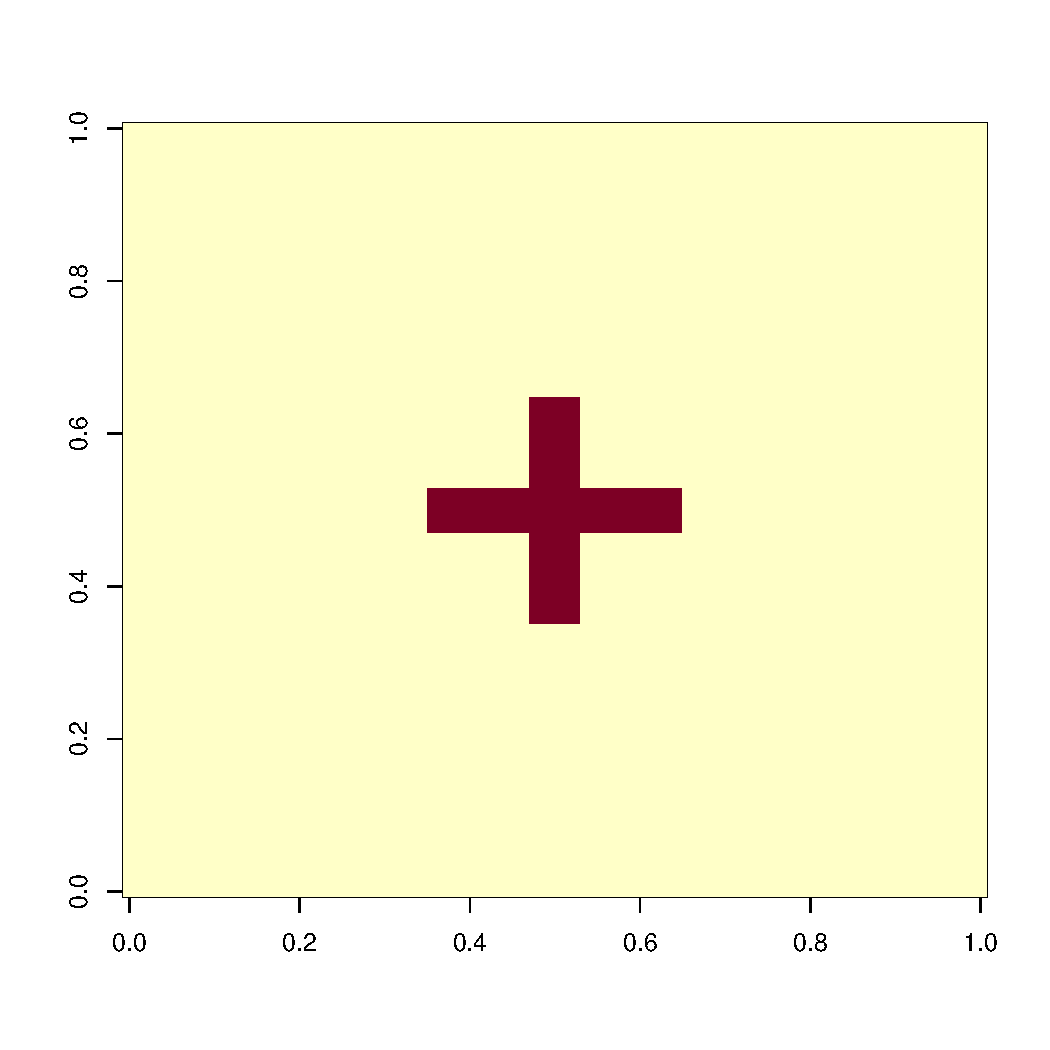
\includegraphics[width=3.8cm]{cross.pdf}
      \includegraphics[width=3.8cm]{block.pdf}
        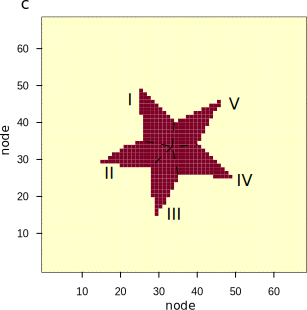
\includegraphics[width=3.8cm]{star.pdf}
          \includegraphics[width=4.7cm]{circle.pdf}
            
          \caption{Four active pattern in simulations. The active region is divided into four or five subregions (denoted I, II, ...), each of which has its own edge connectivity signal $g_{pq}(\pi)$.}\label{fig:region}
\end{figure}

For fair comparison, we adopt similar simulation setup as in~\cite{relion2019network}, except that we add more challenging network patterns in order to assess model misspecification. We simulate the data $(\mX_i, y_i)_{i\in[n]}$ from latent variable model $(\mX,y)|\pi$ based on the following scheme,
\[
\pi \sim_{\text{i.i.d.}} \text{Uniform}[0,1] \stackrel{\text{conditional on $\pi$}}{\longrightarrow}
\begin{cases}
y\sim \text{Ber}(\pi),\ \text{}y\perp \mX|\pi, \\
\mX=\entry{\mX_{pq}}, \ \text{where\ } \mX_{pq}\sim_{\text{i.i.d.}} \tN(g_{pq}(\pi)\mathds{1}(\text{edge $(p,q)$ is active}), \sigma^2).
\end{cases}
\]
The edge connectivity signal, $g_{pq}(\pi)$, varies depending on the response probability $\pi$ and location of $(p,q)\in[d]^2$. Figure~\ref{fig:region} illustrates the active pattern which specifies the locations of active edges. The active region is further divided into several subregions, each of which has its own signal function $g_{pq}(\cdot)\colon [0,1]\to \mathbb{R}$. The function form of $g_{pq}(\cdot)$ is randomly drawn from a pre-specified library consisting of common functions such as $g(z)=\log(5z+1), 3\tan(z),6z^2,\ldots$. We set $d=68$, a training size $n=160$, and a test size $80$. 

Our simulation reflects the challenging heterogeneity commonly arisen in brain network analysis. The sample consists of a mixture of individual groups with varying disease propensity, and the network patterns vary from one group to another. Active brain regions are supported on a submatrix with typically unknown rank. In the noiseless case, the cross and block patterns are low-rank ($r = 3$ and 5, respectively), whereas the star and circle patterns are nearly full-rank (numerical rank $r\approx 30$ on the supported submatrix). In our simulation with noisy observation, we select the rank and sparsity parameters $(r,s)$ by 5-fold cross validation within training data. The hyperparameters for the other three methods are selected by either default setting ({\bf \small LogisticM}) or cross validation ({\bf \small Lasso}, {\small \bf CNN}, {\small \bf NonMAR}). We provide each algorithm the labeled networks as inputs after randomly permuting the node indices in the network. Because the software for \LogisticM supports symmetric matrices only, we provide the algorithm ${1\over 2}(\mX+\mX^T)$. 

\begin{figure}[ht]
    \centering
    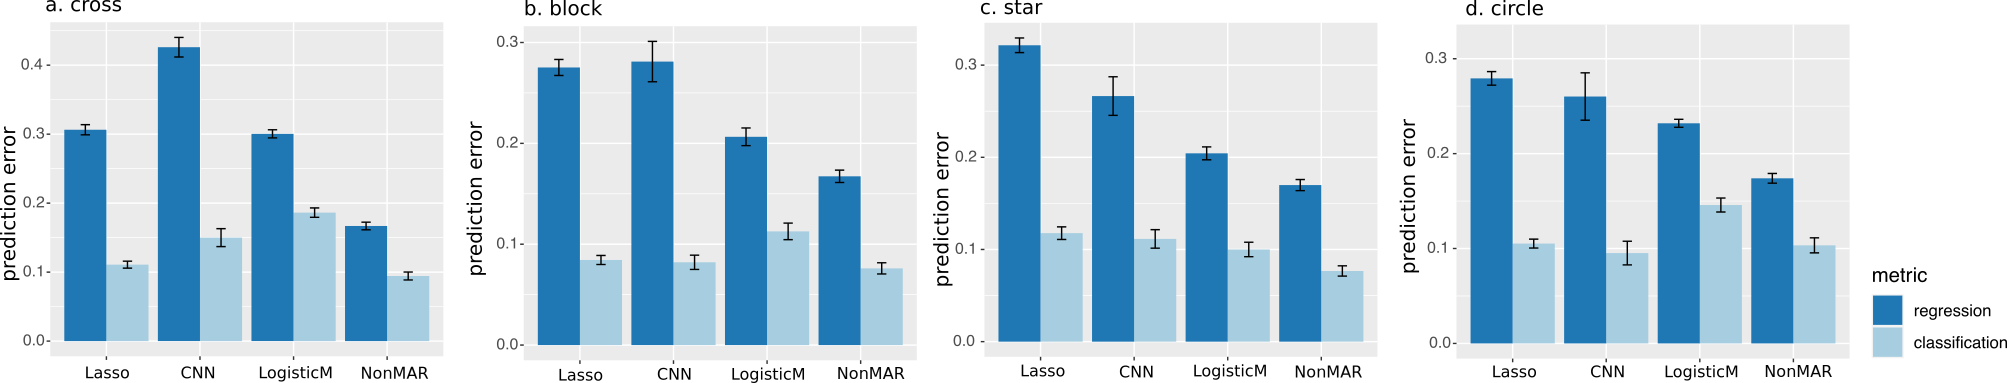
\includegraphics[width=\textwidth]{error_tot_comb2.pdf}
    \caption{Performance comparison between various methods under four different active patterns. }\label{fig:compare}
\end{figure}

Figure~\ref{fig:compare} compares the out-of-sample prediction between different methods. We focus on the regression problem and assess the performance using test data. We find that \NonparaM consistently outperforms others, and the reduction in error is substantial. For example, the relative reduction using \NonparaM over the next best approach, {\bf \small LogisticM}, is over 20\% for patterns a and d, and over 15\% for patterns b and c. The results show the benefit of our nonparametric approaches by allowing more flexible functional space. Furthermore, we find that neither \Lasso nor \CNN has satisfactory regression performance. One possible reason is that these two methods fail to appropriately incorporate the network structure of the predictors. The \Lasso takes vectorized matrices as inputs and therefore losses the two-way pairing information. On the other hand, \CNN assumes spacial ordering within row/column indices. Although local similarity is an appropriate model for common imaging analysis, the row/column indices are meaningless for networks. Indeed, adjacency matrices differ by row/column permutation represent the same network, and methods that are index-invariant (\LogisticM and {\bf \small NonMAR}) show better performance. Our simulations cover a reasonably broad range of network models with rich structure. The results demonstrate the advantages of our nonparametric approach on the task of network regression. 

We also report the accuracy on classification which is an intermediate step of regression. Figure~\ref{fig:compare} shows the favorable performance of our method especially when compared to {\bf \small LogisticM}. Among the four models of active regions, our method performs the best in all three. The only exception is the circle pattern where the \CNN has a lower classification error by a slight margin. This is perhaps due to the fact that circle pattern is nearly full rank which favors complicated models such as {\bf \small CNN}. Nevertheless, our method \NonparaM achieves stable performance in spite of its simplicity. Interestingly, we find that the benefit of our method is more substantial in regression than in classification. One possible reason is that classification is an easier problem and less sensitive to various approaches. The result also suggests that the main reason of our method's superior regression performance may be attributable to level set aggregations. 

\begin{figure}[ht]
    \centering
   \includegraphics[width=8.1cm]{est_block.pdf}
          \includegraphics[width=8.1cm]{est_circle.pdf}
 \caption{Example outputs returned by {\bf \small NonMAR}. Panels (a) and (c) plot the top edges selected by our method. Panels (b) and (d) are scatter plots of the edge connectivity strength (averaged by subregion) versus the estimated response probability. The ground truth function is depicted in dashed curve.}\label{fig:compare2}
\end{figure}


We provide illustrate examples to show the outputs returned by {\bf \small NonMAR}. Figures~\ref{fig:compare2}a and c plot the top edges selected by \NonparaM based on the moving averages of feature weights $(\hat \mB_\pi)_{\pi\in[0,1]}$ with a window size $\Delta \pi = 0.2$. The selected region agrees well with the ground truth (Figures~\ref{fig:compare}a and c). We also investigate the relationship between edge connectivity for individual $i$ and the estimated response probability $\hat \pi_i$. The trajectory of the edge connectivity accurately resembles the ground truth function in each subregion. The results demonstrate that our method is able to recover the right ``sorting'' of individuals with respect to the response probability on a continuous spectrum. 
The successful recovery of complicated unknown functions makes our method {\bf \small NonMAR} appealing in applications. 

\section{Application to human brain connectome data}\label{sec:real}

We apply our method to brain network data from Human Connectome Project (HCP). We analyze the Variable Short Penn Line Orientation Test (VSPLOT) score which measures the individual's visuospatial processing ability. We preprocess the data as in~\cite{wang2019common}, and analyze $n=212$ individuals whose VSPLOT scores are either high ($y=1$) or low ($y=-1$). Each individual's brain network is represented by a 68-by-68 binary adjacency matrix $\mX\in\{0,1\}^{68\times 68}$, with the entries encoding the presence or absence of fiber connections between the 68 brain nodes. We adjust age and gender as additional covariates in the prediction, and use a random 60-20-20 split of the data for training, validation, and testing. 

\begin{figure}[ht]
    \centering
       \includegraphics[width=\textwidth]{braintable.pdf}
 \caption{HCP analysis results based on our method {\bf \small NonMAR}. (a) Comparison of prediction accuracy. (b) Top edges selected by our method {\small \bf NonMAR-p}. }\label{fig:real}
\end{figure}

We compare our performance to other methods using the same procedure as in the previous section. Figure~\ref{fig:real}a shows that our method achieves high regression accuracy, measured by area under receiver operating characteristic (AUC). As common in high-dimensional settings, we observe that models with optimal cross-validation accuracy tend to include many noise variables. A useful heuristic is the so-called ``one-standard-error rule''~\citep{hastie2015statistical}, in which one selects the most parsimonious model with cross-validation accuracy within one standard error of the best. We apply this rule and report the results as {\bf \small NonMAR-p}. It is remarkable to see that {\bf \small NonMAR-p} results in 12\% reduction of active nodes but still achieves excellent accuracy (AUC = 0.73). 


Figure~\ref{fig:real}b lists the top brain edges identified by our method. Edges are ranked by their maximal values in the feature weights $(\hat \mB_\pi)_{\pi \in [0,1]}$ via moving averaging. We find that the top edges involve connections between frontal and occipital regions in the right hemisphere (Figure~\ref{fig:real2}a). This seems consistent with recent evidence of dysfunction in right posterior regions for deficits in visuospatial processing~\citep{wang2019common}. We also find nonlinear relationship between edge connection strength and response probability. In Figure~\ref{fig:real2}b, the connection (r-parstriangularis, r-supramarginal) grows slowly when $\pi$ is low but fast when $\pi$ is high. In contrary, the connection (r-posteriorcingulate, r-precentral) grows fast initially and then reaches a plateau as $\pi$ increaases. The detected pattern reveals the heterogeneous changes in brain connectivities with respect to visuospatial processing ability. 

\begin{figure}[ht]
    \centering
       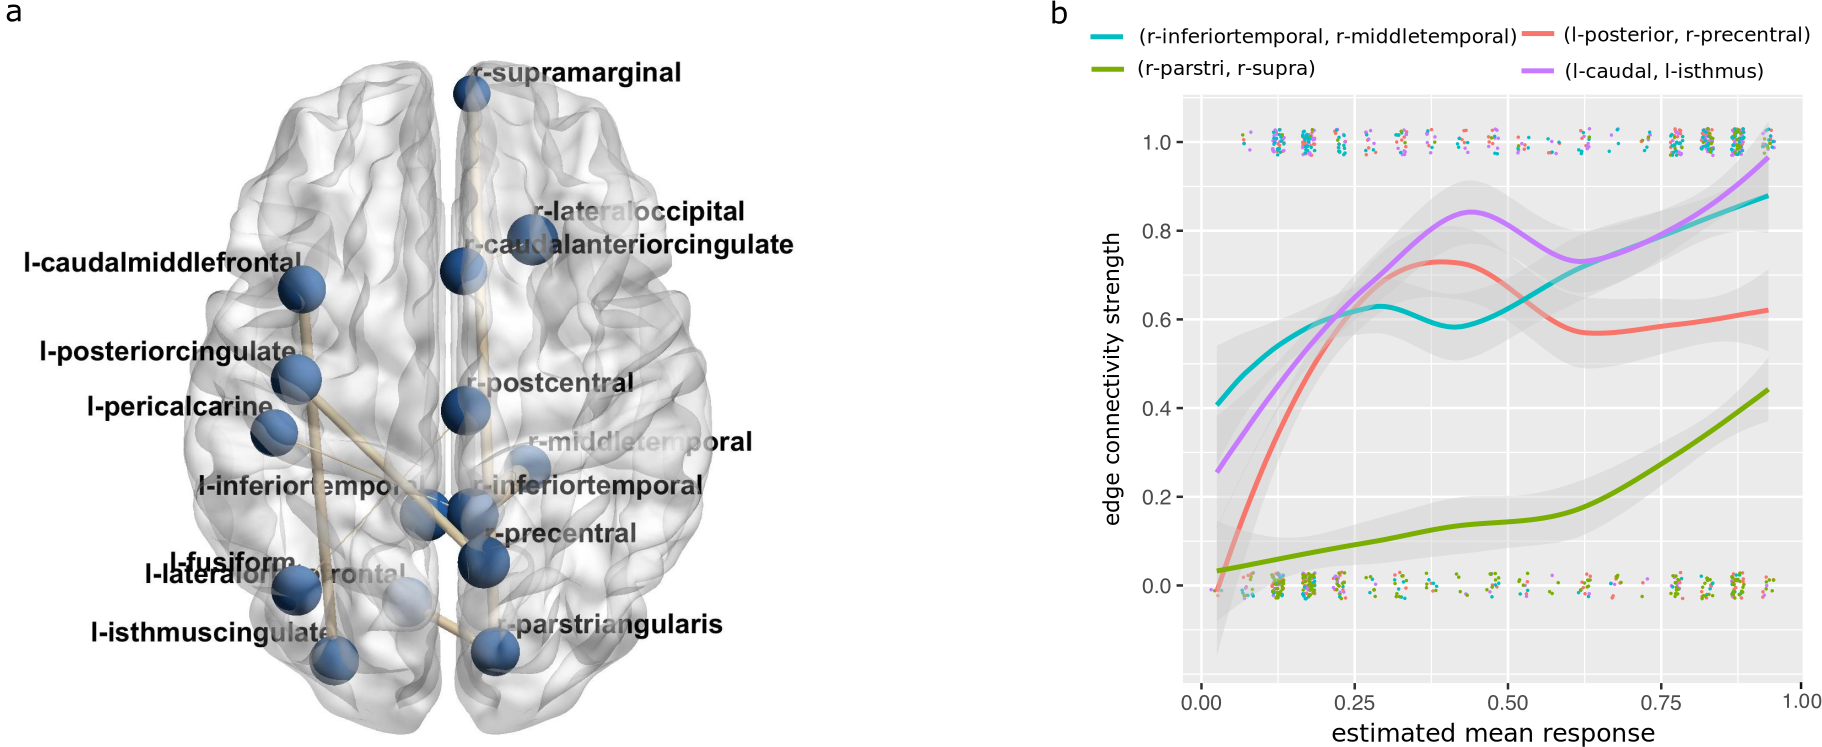
\includegraphics[width=1\textwidth]{brain.pdf}
 \caption{HCP analysis results. (a) Top edges overlaid on brain template. (b) Edge connectivity strength versus estimated response probability. Colored curves represent the moving averages of connectivity strengths, gray bands represent one standard error, and jitter points represent the raw connectivity values (0 or 1). }\label{fig:real2}
\end{figure}



\section{Conclusion}
We have developed the learning framework for the relationship between a binary label response and a high-dimensional matrix-valued predictor. 
Our method respects the matrix structure of the predictors and provide interpretable prediction via a nonparametric approach. 
The theoretical and numerical results demonstrate the competitive performance of our method.
The work unlocks several directions of future research. Extension to multilclass probability estimation and to nonlinear boundaries through kernel methods would be of interest. Application to nonparametic way such as matrix completion and denoising problem warrants future research.


\bibliographystyle{chicago}

\bibliography{tensor_wang}



\end{document}



